\documentclass[addpoints]{exam}

\usepackage{enumitem}
\usepackage{graphbox}
\usepackage{tabularx}
\usepackage{url}

\graphicspath{{images/}}


% Header and footer.
\pagestyle{headandfoot}
\runningheadrule
\runningfootrule
\runningheader{CS 440}{HW I: Foundations I}{Fall 2020}
\runningfooter{}{Page \thepage\ of \numpages}{}
\firstpageheader{}{}{}

\qformat{{\large\bf \thequestion. \thequestiontitle}\hfill[\totalpoints\ points]}
\boxedpoints

\title{Homework I: Foundations I}
\author{CS 440 Computer Graphics\\Habib University\\Fall 2020}
\date{Due: 18h on Friday, 11 September}

\begin{document}
\maketitle

\begin{questions}

\titledquestion{MyImage}[0]

  \noindent\begin{tabularx}{\textwidth}{lX}
    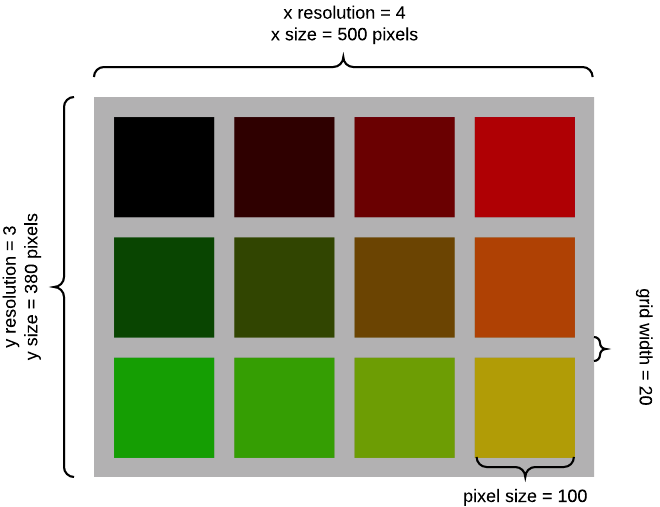
\includegraphics[width=.45\textwidth,align=t]{demo} &

    The attached file, \texttt{MyImage.py}, defines a class \texttt{MyImage} to support basic image manipulation. The image consists of virtual pixels separated by gridlines. The size of each virtual pixel may be larger than a screen pixel. For example, the \texttt{MyImage} instance on the left has a resolution of 4x3 virtual pixels. The size of each virtual pixel is 100 pixels, and the width of gridlines is 20 pixels. The actual raster ends up being 500x380 pixels.

    Methods are included in the class to create an image from scratch, read an image from file, display the image, get/set pixel colors, and provide other functionality. A test function is included in the file. You will be using this class in this and the next assignment.
  \end{tabularx}

  \underline{Task}: Go over the file \texttt{MyImage.py} to gain an understanding of the class and its methods. Feel free to write your own tests.

\titledquestion{Blow It Up}[10]

  \begin{tabularx}{\textwidth}{cX}
    
\includegraphics[align=t]{logo} & We will work on the image on the left, included as \texttt{images/logo.png}, in this question. We will read the image into a \texttt{MyImage} instance and display blown up versions of it using another \texttt{MyImage} instance which has the same resolution, twice the pixel size, and grid lines of width 1. We will blow it up in five different ways. The first four will display a) exactly the same, b) only red, c) only green, and d) only blue, colors from the original image.
  \end{tabularx}
  The last blowup e) displays a CMY version. That is, each RGBA color value from the original image is interpreted as a CMYK value instead.
  \begin{center}
    \begin{tabular}{*{5}{c}}
      
\includegraphics[width=.16\textwidth]{blow}
      & 
\includegraphics[width=.16\textwidth]{logo-r}
      & 
\includegraphics[width=.16\textwidth]{logo-g}
      & 
\includegraphics[width=.16\textwidth]{logo-b}
      & 
\includegraphics[width=.16\textwidth]{logo-cmy}
      \\ a) blow* & b) red* & c) green* & d) blue* & e) cmy*
      \\\multicolumn{5}{l}{*-- image scaled down from actual size.}
    \end{tabular}
  \end{center}
  \underline{Task}: Write a function, \texttt{blow()}, that takes the path to an image file as argument and displays the above blowups of the image one after the other.\\
  \underline{Note}: The read image will have a value of 255 for Alpha. Using that value for K in CMYK will cause the pixel to appear black so you will have to adjust for that. 
  
\titledquestion{Bilinear Interpolation}[5]
  \noindent\begin{tabularx}{\textwidth}{lX}
    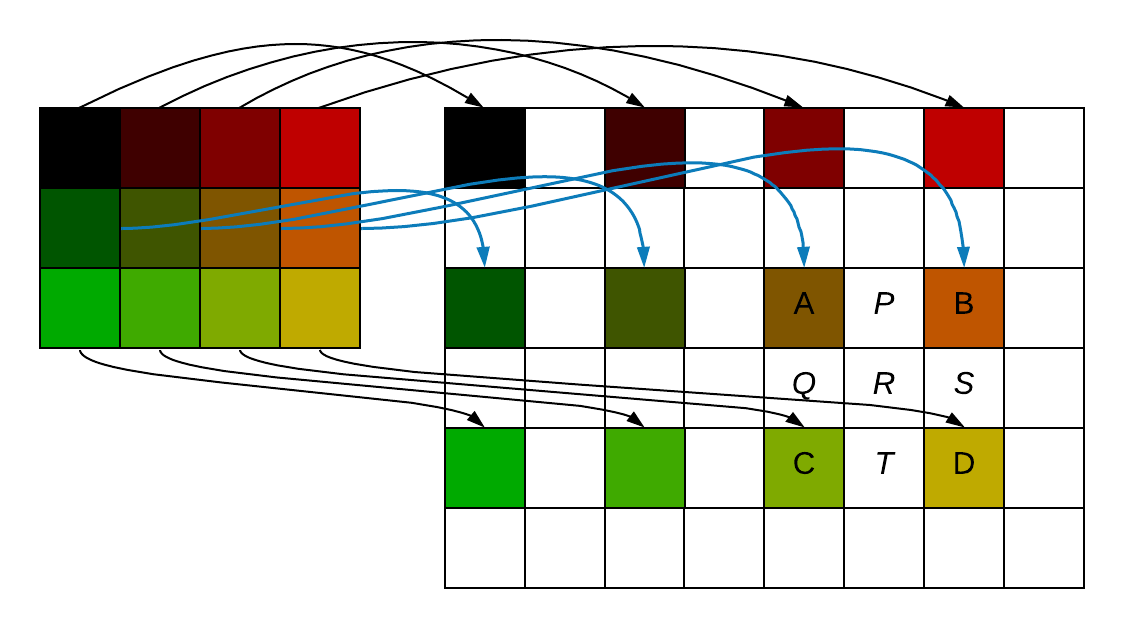
\includegraphics[width=.4\textwidth, align=t]{resize}
    & 
    Consider the case below where a 4x3 image is resized to twice its size. The resized image has 4 times as many pixels and some of them take on the values from the original image as shown. For the pixels shown to be blank, color values are not known and have to be computed from the known values. 
    Consider the labeled pixels in the resized image above. One way to fill in the missing color information is as follows.
    \[
      P = \frac{1}{2}(A + B),\; T = \frac{1}{2}(C + D),\; Q = \frac{1}{2}(A + C),\; S = \frac{1}{2}(B + D)
    \]
  \end{tabularx}
  There are various ways to compute R, all of which are ultimately equivalent.
  \[
    R = \frac{1}{2}(P + T) = \frac{1}{2}(S + Q) =  \frac{1}{4}(A + B + C + D) = \frac{1}{4}(P + Q + S + T) = \frac{1}{8}(A + B + C + D + P + Q + S + T)
  \]
  The boundary pixels pose a problem as some of the neighboring pixels required for the average do not exist. In such cases, only the existing neighbors are used for the average.

  Notice how all the above expressions are affine combinations. Furthermore, the colors for P, Q, S, and T are \textit{linearly interpolated} from their horizontal or vertical neighbors. The color for R is a \textit{bilinear interpolation}: it is a linear interpolation of P and T, or Q and S, which are themselves linear interpolations.

  \underline{Task}: Write a function, \texttt{resize()}, that takes the path to an image file as argument and displays the image and its resized version one after the other.\\
  \underline{Note}: For the purpose of \texttt{MyImage}, all divisions in the above expressions are integer divisions.
  
  
\titledquestion{Sierpinski Triangle}[5]

  \begin{tabularx}{\linewidth}{cX}
    
\includegraphics[scale=0.75, align=t]{sierpinski}
    & The Sierpinski triangle is an interesting pattern that arises in many different ways. We will use the \textit{chaos game} construction which proceeds as follows.\footnote{\url{https://en.wikipedia.org/wiki/Sierpiński_triangle}}\newline
    1. Take three points in a plane to form a triangle, you need not draw it.\newline
    2. Randomly select any point inside the triangle and consider that your current position.\newline
    3. Randomly select any one of the three vertex points.\newline
    4. Move half the distance from your current position to the selected vertex.\newline
    5. Plot the current position.\newline
    6. Repeat from step 3.
  \end{tabularx}

  \underline{Task}: Write a function {\tt sierpinski} that takes as arguments: a \texttt{MyImage} instance, \texttt{img}; an \texttt{int}, \texttt{n}; and 3 integer pairs. Each pair represents the coordinates of a virtual pixel in \texttt{img}. The function performs \texttt{n} iterations of the chaos game, plots the resulting points in \texttt{img}, and displays the resulting image.
  
  
\end{questions}

\end{document}
%%% Local Variables:
%%% mode: latex
%%% TeX-master: t
%%% End:
